%% This document gives an example on how to use the ntnubachelorthesis
%% LaTeX document class.
%% Use oneside for PDF delivery and twoside for printing in a book style
%% use language english, norsk, nynorsk and one of the following shortenings
%%  ``BSP'' Bachelor i Spillprogrammering,\\
%%  ``BRD'' Bachelor i drift av nettverk og datasystemer,\\
%%  ``BIS'' Bachelor i Informasjonssikkerhet,\\
%%  ``BPU'' Bachelor i Programvareutvikling, \\
%%  ``BIND'' Bachelor i Ingeniorfad - data, \\
%%  ``BADR'' Bachelor i drift av datasystemer, \\
%%  ``BIT'' Bachelor i informatikk, \\
%%  ``BABED'' Bachelor i IT-støttet bedriftsutvikling.
%%   for example \documentclass[BIS,norsk,twoside]{ntnuthesis/ntnubachelorthesis}

\documentclass[BSP,english,oneside]{ntnuthesis/ntnubachelorthesis}

\usepackage{csvsimple}
\usepackage{booktabs}
\usepackage{minted}
\usepackage{pdfpages}

\newcommand{\comment}[1]{\textcolor{blue}{\emph{#1}}}  %% use of the colour and you can see how to use commands with parts \comment{so what}

%% The class files defines these two
%% \newcommand{\NTNU}{Norwegian University for Science and Technology} %

% you can create you one #define like structures using the \newcommand feature
% you can change behaviour using \renewcommand

\newcommand{\com}[1]{{\color{red}#1}} % supervisor comment
%\renewcommand{\com}[1]{} %remove starting % to remove supervisor comments
% This will appear in text \com{Lecuters comment} and be visible unless you uncomment
% the renewcommand line.

\newcommand{\todo}[1]{{\color{green}#1}} % items to do
%\renewcommand{\todo}[1]{} %remove starting % to remove items to do

\newcommand{\n}[1]{{\color{blue}#1}} % other comment
%\renewcommand{\n}[1]{} %remove starting % to remove notes

\newcommand{\dn}[1]{} % add the d to a note to say that you have finished with it.


% Norwegian Characters,  needs the {} or to be separate from the next letters
% \o{}   \aa{}   \ae{}   so at the end of a word you can use \o  \aa   \ae
% \O{}   \AA{}   \AE{}   you can also just leave a space and latex will remove it
%    eg, NTNU i Gj\o vik  or NTNU i Gj\o{}vik

\begin{document}

\thesistitle{Conductor Hero - Project Report}
%\thesisshorttitle{} % use this if you have a very long title and want something shorter on the header pages
\thesisauthor{Rikhart Vigdal Bekkevold} %thesisauthorA, B, C etc
\thesisauthorA{Sabina Niewiadomska}
\thesisauthorB{Per-Morten Straume}
\thesisauthorC{Ida Ellinor Syverinsen}
\thesisauthorD{Andreas Wang}
\thesisauthorE{Yijie Zhou}

\nmtkeywords{Project Report, Virtual Reality, SteamVR, Unity Engine, ~Interaction Design, Game Design, 3D Modelling}

% Note: this can only be one paragraph with this template
\nmtdesc{
Experts in Teamwork is a course where students from various disciplines are put together in a team to work on a project throughout the semester. For the course, our group worked on a VR game called Conductor Hero where the player takes the role of a Conductor in a fantasy environment. The development of this project has taught us the importance of working with tight schedules as well as provided experience with cross disciplinary teams. The project report for Conductor Hero contains the technical details and methods for how the game was developed as well as discussions around the decisions that led to the final product. 
}


\nmtoppdragsgiver{\NTNU}
% TODO: Maybe this should be replaced by Sabina since she is PR
\nmtcontact{Andreas Wang, andrwan@stud.ntnu.no, 48048162}

\thesisdate{\ntnubachelorthesisdate}
\useyear{04.05.2018}

\nmtappnumber{1} %number of appendixes
\nmtpagecount{} %currently auto calculated but might be wrong % this is the file which contains all the details about your thesis

\makefrontpages % make the frontpages

\tableofcontents
\listoffigures
%\listoftables
%\listoflistings

\chapter{Introduction}
\chapter{Methods} \label{chap:methods}
\section{Idea Generation} 
The idea generation followed a ''divergent - emergent - convergent'' process~\cite{gameBook}, as shown in Figure~\ref{fig:ideaGeneration}. At the first stage, we conducted a brainstorming session, where each group member freely expressed their ideas related to VR and AR in the field of games, health or education. A range of ideas was generated, including a rehearsal room for musicians or dancing classes, a public speaking practice place, collaborative painting or sand painting, a virtual memory palace, a 3D-data visualisation room and simulators for activities like gardening, parachuting or car racing. 

After discussing all ideas we decided to apply dot-voting~\cite{gameBook} which helped us to prioritize our favourite ideas. All of us received three votes and we were asked to distribute the votes (dots) as we saw fit. This meant that we could put all three dots on one of the ideas or we could put one dot on three different ideas instead. When everyone had placed all their dots, we narrowed our focus to the three ideas with the most votes. 

One of the ideas was to create a service which lets the musicians or DJs play their own music and artists to display visualisations, while an audience could meet in virtual space to experience the audio-visual performance and dance together. Another was an educational chemistry game, aimed at school children. The final idea was to create an orchestral conducting game.

\begin{figure}[tbph]
    \centering
    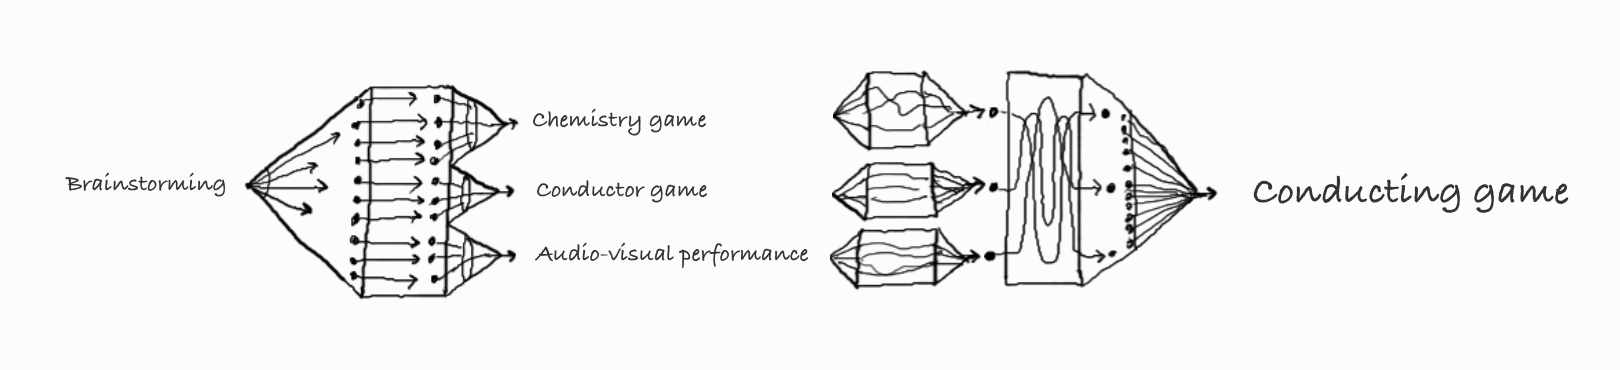
\includegraphics[width=1.0\textwidth]{images/ideaGenerationProcess.png}
    \caption[Idea Generation Process]{The process of idea generation~\cite{gameBook}}
    \label{fig:ideaGeneration}
\end{figure}

In the following discussion of these ideas, we sketched the scenarios of the games, as well as the implementation details. We now had a better feel for, and understanding of, each idea. Together we decided that we would like to try to develop the orchestra conductor game. Among the reasons for this choice was the strong musical background of four group members, as we believed our musical experience would help us to create a more interesting game scenario. The lack of market competitors also played a part in our decision, additionally, the VR technology seemed to suit conducting well. Sketching of ideas was further used in the project to illustrate our ideas to each other as shown in Figure~\ref{fig:tablesketch} which contains a sketch of how we envisioned the various elements of the Conductor Table. 

\begin{figure}[tbph]
    \centering
    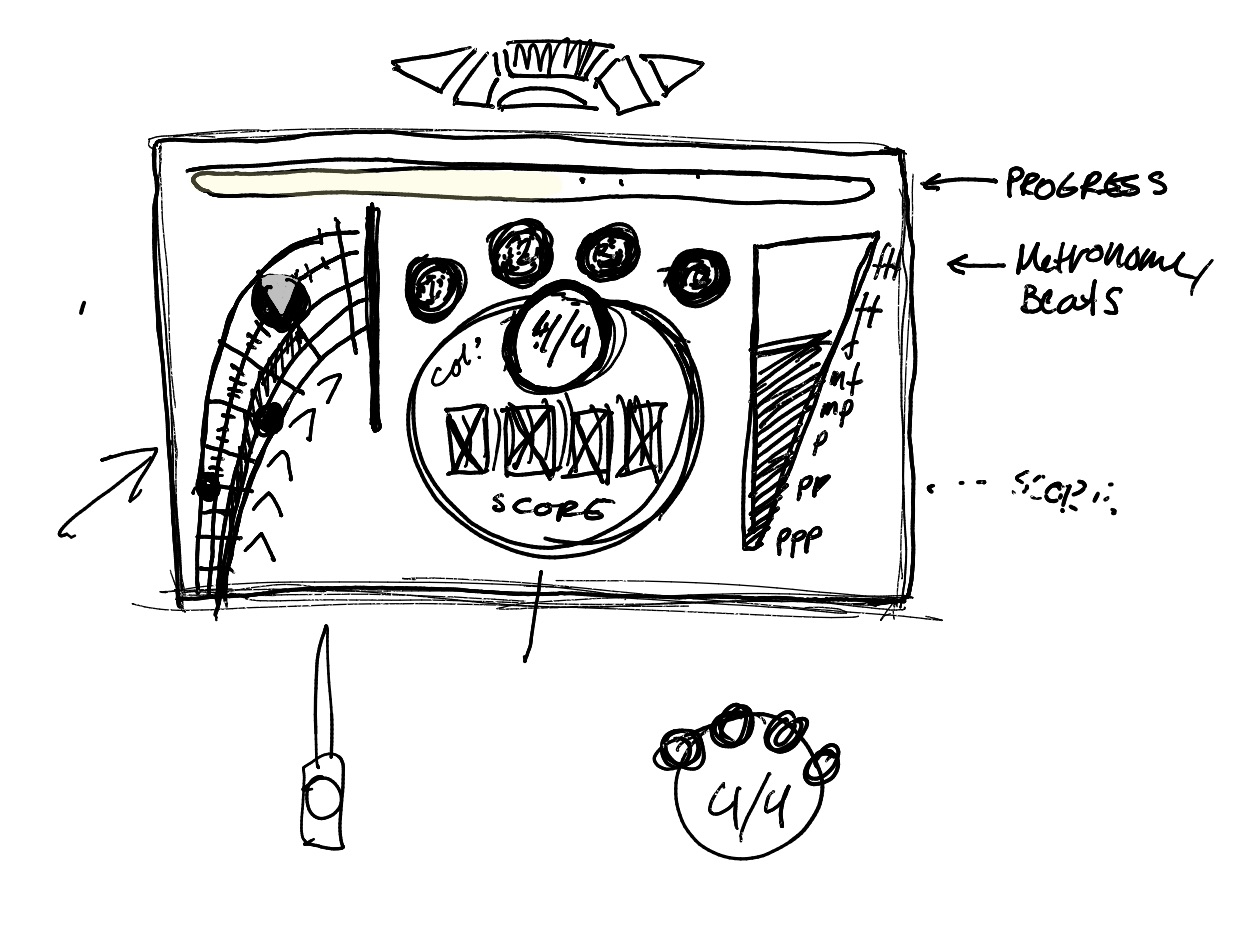
\includegraphics[width=0.75\textwidth]{images/sketch.jpg}
    \caption[Example sketch of the Conductor Table]{An initial concept sketch from the development of the Conductor Table.}
    \label{fig:tablesketch}
\end{figure}

\section{Interview}
After choosing to develop a conducting game, we interviewed a professional conductor over Skype to learn more about his experience of conducting and conductor training. The purpose of the interview was to better understand the different aspects of conducting. We also wanted to explore possibilities of involving VR games to promote the positive sides of conducting and to make any negative sides of the training process seem more engaging. During the interview, we found one motivation for the role of conducting, which is the feeling of control and leadership, as the orchestra follows your directions. It is relatively hard to get access to a whole orchestra for conducting training in real life, especially for conducting fanciers or novices. However, in a VR environment, it is possible to have access to a virtual orchestra with a customized composition at any time as long as the player has access to a VR device. With the interactions and feedback from the virtual orchestra, players can achieve greater motivation to keep on training. From the interview, we also got the idea that using unique virtual environments and game elements may ease the feeling of dullness and stress during repeated training. The feedback from the conducting expert confirmed pre-existing assumptions for the features in the conductor game and helped us to have a clearer vision about potential users.

\section{Tools}
The game was created using the Unity engine (version 2017.3.0.3f) with C\# as a language for the scripting components. Microsoft's Visual Studio 2017 Community was used as the Integrated Development Environment. Version control was done through Git using Github as our hosting service. Google drive was used for storing sound files, as these came close exceeding Github’s restrictions on file size, and to a large extent slowed the system down.
Valve’s Unity SteamVR plugin was used for communicating with the HTC Vive. Blender was used for modeling 3D assets, like the instruments and game world. The UI for the conducting table was created with Adobe Illustrator and Adobe Photoshop. The soundtrack used for the game was composed in Guitar Pro 5. Cubase 5 was used as the Digital Audio Workstation when generating audio from the midi tracks exported from Guitar Pro 5, using Virtual Studio Technology instruments from EastWest/Quantum Leap symphonic orchestra to produce the desired individual instrument tracks. Discord was used for intragroup communication.


\section{Development Methodologies}
The development followed a mixed methodology model with a focus on aspects that would allow us to work in parallel and quickly prototype features. Code hygiene factors was a low priority due to the limited time and we did not expect that performance would be an issue with such a limited game. We, therefore, adopted a ''critical path coding''~\cite{critical_path_coding} approach to get as much done with as little code as possible.

Developers usually worked individually after short discussions on architecture, however, pair programming techniques were employed for more challenging or unfamiliar problems. 
We originally intended to have a focus on the process, making proper use of issue tracking, branching strategies, and code reviews. However, early in the project, we came to the conclusion that this added unnecessary overhead to a time-limited project. We decided it would be more beneficial for the project that we spent more time on implementation rather than documentation and process.

In terms of meetings, we employed daily three minute meetings during the morning of every village day in a similar vein to those used in agile software methodologies. These meetings consisted of every group member mentioning any additional progress that had happened since the last day, what they planned to work on during the village day and discussing any potential problems that may arise. We kept these meetings to a maximum of three minutes per group member as a means to avoid situations where certain group members could end up dominating the discussions.
\chapter{Results} \label{chap:results}

\section{Game Design Document}
We generated an initial design document for the game, giving a brief overview of the envisioned game, and a plan for the game mechanics. This document can be found in the Appendix \ref{chap:appendix}.

\section{Game Implementation}
After creating the game design document we implemented a functional prototype of the conductor hero game. The source code and binaries are located on github\footnote{\url{https://github.com/Per-Morten/imt4310_conductor_hero}}. In order to play the game, a functioning HTC Vive headset is required. Instructions on how to install and play the game can be found on the main GitHub repository page. A youtube video\footnote{\url{https://www.youtube.com/watch?v=YQQTDyfQb-Q}} was recorded to demonstrate the features of the game.

\subsection{Asset Attribution}
The majority of assets used in Conductor Hero were created by us with a few exceptions:
\begin{itemize}
\item Particle Fog textures were acquired from Unity’s Standard Assets.
\item The skybox used in the game was acquired from the Unity Asset Store\footnote{\url{ https://assetstore.unity.com/packages/2d/textures-materials/sky/10-skyboxes-pack-day-night-32236}}   
\item The models for the HTC Vive Controllers were provided with the SteamVR plugin. 
\item The font used in the Conductor Table was acquired from dafont\footnote{\url{ https://www.dafont.com/white-rabbit.font}}. 
\end{itemize}

\subsection{Core Game Components}
The four core components that make up the game are: GameManager, Metronome, AudioManager, and MotionTracker.

The GameManager component manages musical cues as well as scoring. The Metronome component handles the core beat logic. It allows outside components to ask how close they are to being on beat. Other components can also add callbacks to the metronome which will be called every beat. The default sound for the metronome was removed, partly due to uncertainties regarding licensing. The AudioManager manages simultaneous playback of the multiple instrument tracks, metadata about song length and supports muting and unmuting individual tracks. 

Finally, the MotionTracker component handles game logic related to the right hand conducting. This includes managing the visuals of the pattern and any logic for tracking the player’s movement within the pattern, using the tracking spheres in the scene.  

\subsection{Standard game flow} 
The following section describes the standard game flow in the prototype level of Conductor Hero:
\begin{itemize}
\item The player starts the game and the stage will go to an unlit state.  
\item The two controllers are separated by having one with a laser pointer and one without. The “laser pointer” on one of the controllers indicates that it should be held in the left hand.
\item In order to start the game, the player needs to hold their right controller in an upwards position where they would feel comfortable having the top of the conducting pattern and press the menu button to start. 
The game starts a countdown to the song which ends with the first cue.
\item While playing, the player’s left hand is used to hit cues on beat while their right hand is used to keep the conducting pattern going. 
    \begin{itemize}
    \item[--] A cue appears at designated times during the song. The cue has a circular progress bar which implies when the player is supposed to hit it.
    \end{itemize}
\item The game ends when the song is finished.
\end{itemize}

\subsection{Shortcomings of the Prototype}
In the prototype, the game will start the countdown to the song and show the pattern to the player, but currently, it will also start counting score for movement even if the song has not properly started yet. This is unintended as we would like to start measuring score after the first cue, but we did not have the time to fix this by the end of the project. The game is also supposed to end once the song duration has expired, but we do not have any additional end states to signify this due to time constraints.  

\subsection{Playtesting}
As part of the development, we performed a lot of internal testing within the development team. We also had an initial playtesting session with the entire group and also asked some members of other teams to try out the game and give feedback. This playtesting session is further discussed in the Discussion Chapter.

\section{Presentation}
As part of the course, we also had a presentation towards the end where we showed off the project to the class, the supervisor and industry externals. The slides from the presentation can be found on Google Slides~\footnote{\url{https://docs.google.com/presentation/d/1unr5goORWJpajkHhiNFVHJUfyByFeLB_AzXME653Kd0/edit?usp=sharing}}
\chapter{Discussion} \label{chap:discussion}

\chapter{Conclusion}


\bibliographystyle{ntnuthesis/ntnubachelorthesis}
\bibliography{inc/BachelorExample}

\appendix %after this line all chapters will have letters instead of numbers
% spreadsheet data?

\end{document}
